\documentclass{standalone}
\usepackage{tikz}
\usepackage{amsmath}

\begin{document}
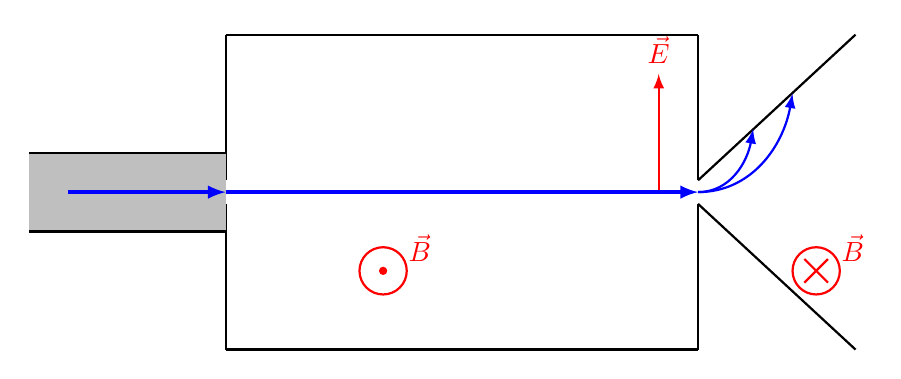
\begin{tikzpicture}

    % Dibujar el rectángulo grande (selector) con una apertura
    \draw[thick] (0,0) -- (0,1.85);
    \draw[thick] (0,2.15) -- (0,4);
    \draw[thick] (6,2.15) -- (6,4);
    \draw[thick] (6,1.85) -- (6,0);
    \draw[thick] (0,4) -- (6,4);
    \draw[thick] (0,0) -- (6,0);

    % Campo eléctrico E (flecha hacia arriba)
    \draw[red,thick,-latex] (5.5,2) -- (5.5,3.5) node[above] {$\vec{E}$};
    
    % Campo magnético B (círculo con un punto, campo hacia afuera)
    \draw[red,thick] (2,1) circle (0.3);
    \fill[red] (2,1) circle (1.5pt); % Punto en el centro
    \node[red,above right] at (2.2,1) {$\vec{B}$};

        % Campo magnético B (cruz roja pequeña)
    \draw[red,thick] (7.5,1) circle (0.3);
    \draw[red,thick] (7.5-0.15,1-0.15) -- (7.5+0.15,1+0.15);
    \draw[red,thick] (7.5-0.15,1+0.15) -- (7.5+0.15,1-0.15);
    \node[red,above right] at (7.7,1) {$\vec{B}$};

    % Dibujar las paredes de entrada (rectángulo pequeño) con relleno gris claro y apertura
   \fill[lightgray] (-2.5,2.5) rectangle (0,1.5);
    
    % Dibujar los bordes del rectángulo pequeño con la apertura
    \draw[thick] (-2.5,2.5) -- (0,2.5);
    \draw[thick] (-2.5,1.5) -- (0,1.5);
    
    % Trazo de partículas que entran al selector
    \draw[very thick,blue,-latex] (-2,2) -- (0,2);
    \draw[very thick,blue,-latex] (0,2) -- (6,2);

    %Detector
    \draw[thick] (6,2.15) -- (8,4);
    \draw[thick] (6,1.85) -- (8,0);

    \draw[thick, -latex, blue] (6,2) to[out=0, in=260](6.7,2.8);
    \draw[thick, -latex, blue] (6,2) to[out=0, in=260](7.2,3.25);
\end{tikzpicture}
\end{document}
